% inspired from http://tex.stackexchange.com/questions/57152/how-to-draw-graphs-in-latex
\documentclass{article}
\thispagestyle{empty}

\usepackage{tikz}
\usetikzlibrary{positioning}
\usetikzlibrary{arrows}

\begin{document}

% Exemple de cycle améliorant

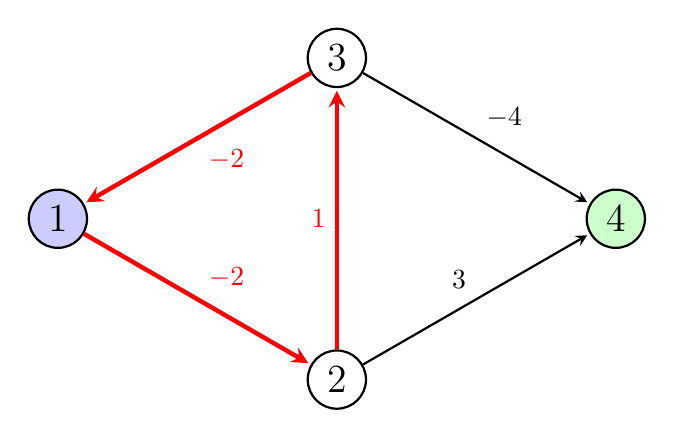
\begin{tikzpicture}[ shorten >=1pt, ->, >=stealth, auto, node distance = 3cm, thick, 
   node/.style = {circle, draw,
                     font = \sffamily\Large\bfseries}]
   \node[node, fill = blue!20] (1) {$1$};
   \node[node] (2) [below right = 1.5cm and 3cm of 1]{$2$};
   \node[node] (3) [above right = 1.5cm and 3cm of 1]{$3$};
   \node[node, fill=green!20] (4) [below right = 1.5cm and 3cm of 3]{$4$};

   \path[color = red, ultra thick] (1) edge node {$-2$} (2);
   \path[color = red, ultra thick] (2) edge node {$1$} (3);
   \path (2) edge node {$3$} (4);
   \path[color = red, ultra thick] (3) edge node {$-2$} (1);
   \path (3) edge node {$-4$} (4);
\end{tikzpicture}

\end{document}
